\subsection{Experiment 4: Nonholonomic robots}%
\label{sub:experiment_4_nonholonomic_robots}

\paragraph{Simulation}
This experiment assesses the performance of the proposed method to compute
trajectories for non-holonomic robots with fabrics. Specifically, we run
experiments for a \textit{Clearpath Boxer} for position. As
for the first experiment, we compare the performance to \ac{mpc}. In this
experiment, the initial position, the goal location, and the position of five
obstacles were randomized. The results reveal that our extension of
optimization fabrics to non-holonomic robots maintains similar results as with
a robotic arm. Specifically, computational time can be reduced to
optimization-based methods while maintaining good performance in terms of
safety and goal-reaching, \cref{fig:experiment4_simBoxer}. We can also observe
that success rate with \ac{sf} is lower compare to \ac{mpc} due to a high
number of unreached goals.

\begin{figure}[h]
  \centering
  \begin{subfigure}{1.0\linewidth}
    \centering
    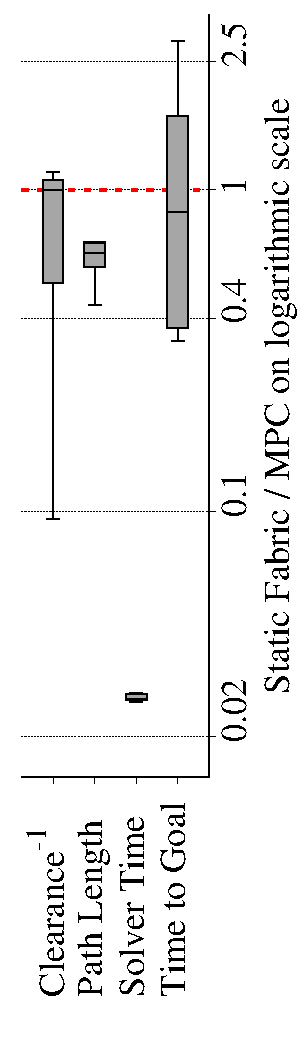
\includegraphics[angle=-90,width=\textwidth]{4_non_holonomic/simBoxer/results_comparison}
    \caption{Metrics evaluation for successful experiments}%
    \label{subfig:experiment4_simBoxer_res}
  \end{subfigure}
  \begin{subfigure}{1.0\linewidth}
    \centering
    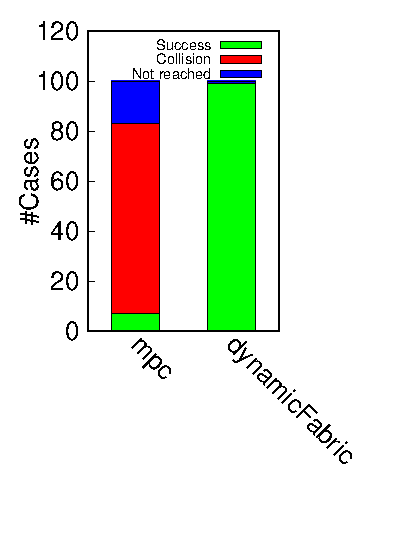
\includegraphics[angle=-90,width=\textwidth]{4_non_holonomic/simBoxer/success}
    \caption{Success results}%
    \label{subfig:experiment4_simBoxer_success}
  \end{subfigure}
  \caption{Results for randomized cased with the Clearpath Boxer robot.
    Similar performance in terms of safety and goal-reaching can be combined with very
    fast computation using optimization fabrics.
  }%
  \label{fig:experiment4_simBoxer}
\end{figure}


